\chapter{Related Work}
\label{chap:related_work}
This chapter gives an overview of the literature on different concept drift detection approaches, state-based process mining and positions the thesis in the literature. Section~\ref{sec:related_work:control_flow} presents detectors that focus on detecting control-flow drifts, and Section~\ref{sec:related_work:perspectives} focuses on the works on detectors beyond control-flow. Section~\ref{sec:related_work:clustering} covers clustering-based detection approaches. Section~\ref{sec:related_work:states} describes the role of states in process mining and reviews the state-based literature. In Section~\ref{sec:related_work:logs} we focus on publicly available event logs with known drifts as test data for the evaluation. Finally, Section~\ref{sec:related_work:positioning} positions this thesis in the literature by explaining similarities and differences of our framework.

\section{Drift Detection in Control-Flow}
\label{sec:related_work:control_flow}
The most common strategy is a statistical test that compares the behavior of neighboring windows. In the survey of \textcite{sato2022survey} 11 out of 36 papers use a statistical test approach. \textcite{bose2011handling} apply statistical tests on follows relationships features between activities. The tool ProDrift developed by \textcite{maaradji2017detecting} uses a $\chi^2$ test on the distribution of partially ordered runs, changes the window size adaptively and detects gradual drifts alongside sudden drifts. ProDrift receives higher F1-scores and detects drifts earlier than the approach of \textcite{bose2011handling}.

Other detectors represent the control-flow differently. In Tsinghua Process Concept Drift Detection (TPCDD) \textcite{zheng2017detecting} derive candidate drift points from a matrix of traces and relations and cluster them together using DBSCAN. With an error tolerance (ET) of 10 traces around the actual drift point, TPCDD achieves an F1-score of 1.0, whereas ProDrift needs an ET of about 100 traces for a comparable score on the same test data. CV4CDD-4D~\autocite{kraus2025machine} learns to detect concept drifts using event logs with known sudden, gradual, incremental, and recurring drifts in an image of window similarities. CV4CDD-4D achieves an F1-score of 0.86 and finds the drift points more granular than the other approaches evaluated. It is also more robust against noise.

Beyond drift detection, \textcite{kraus2026characterization} distinguish drift localization (what changed) from drift characterization (how it changed over time) and address the latter. In our terms, these correspond to drift types and drift modes.

All the detectors consider only the control-flow and therefore just the intra-case perspective of this thesis. Drifts that only change the waiting times, such as the one in Figure~\ref{fig:intro:motivation}, stay hidden.

\section{Drift Detection Beyond Control-Flow}
\label{sec:related_work:perspectives}
Several detectors cover further perspectives. \textcite{brockhoff2020time} compare the trace distribution of two windows using the Earth Mover's Distance (EMD) with regard to processing and sojourn times.

Three detectors detect drift points using the Pruned Exact Linear Time (PELT) algorithm on time series of features. \textcite{adams2023explainable} use control-flow, performance, data, resource, object features and test pairs of detected drifts for Granger causality. \textcite{klijn2024multi} use features on resources and control-flow using an event knowledge graph (EKG). CVDrift by \textcite{khraiwesh2027window} chooses the window size of each time series from its coefficient of variation (CV), with series for control-flow, time, and resources. On event logs with activity duration drifts CVDrift achieves F1-scores from 0.77 to 0.97.

PELT-based detectors observe a drift in many features but capture the inter-case perspective only through individual features such as arrival time or processing time.

\section{Clustering-Based Drift Detection}
\label{sec:related_work:clustering}
Methodologically, the clustering-based detectors are the most similar to this thesis. Clustering-based detectors observe how the composition of clusters changes over time and newly emerging or vanishing clusters are a drift signal (\textcite{sato2022survey}). Concept-Drift in Event Stream Framework (CDESF) developed by \textcite{barbonjunior2018framework} clusters cases of an event stream using DBSCAN with respect to distances in control-flow and time. CDESF signals a drift when outlier cases become dense enough to form a new cluster. Version Clustering (\textcite{abarcazuniga2026version}) clusters windows according to their directly-follows frequencies into process versions using Hierarchical Density-Based Spatial Clustering of Applications with Noise (HDBSCAN). It signals drift points at the transitions between these versions. Using a tolerance of 5\% of the cases, Version Clustering achieves F1-scores of 0.84 and 0.96 on two benchmarks.

Both approaches apply clustering in a feature space describing mostly the control-flow. Version Clustering (\textcite{abarcazuniga2026version}) applies clustering on full windows similar to resource and inter-case perspectives of this thesis, but in our thesis the states do not represent a process version.

\section{States in Process Mining}
\label{sec:related_work:states}
Classically a state describes a running case for making predictions. \textcite{vanderaalst2016process} predicts remaining time of cases using annotated transition systems with states (Figure~\ref{fig:related_work_states_prediction}). \textcite{senderovich2017intra} encode running cases for prediction in a state space from intra-case and inter-case dependencies.

\textcite{berti2025ocel} learn execution states of objects using sliding windows, PCA and SOM. In this thesis, we adapt the approach to cases and extend it to resource and inter-case perspectives beyond the intra-case perspective using calendar windows and feature extraction for concept drift detection.

\textcite{kraus2026steady} detect steady states from KPIs for each time window like the number of active cases. A fluctuating arrival rate is not seen as a concept drift by the paper whereas for this thesis it is a concept drift in the inter-case perspective.

\begin{figure}[tb]
	\centering
	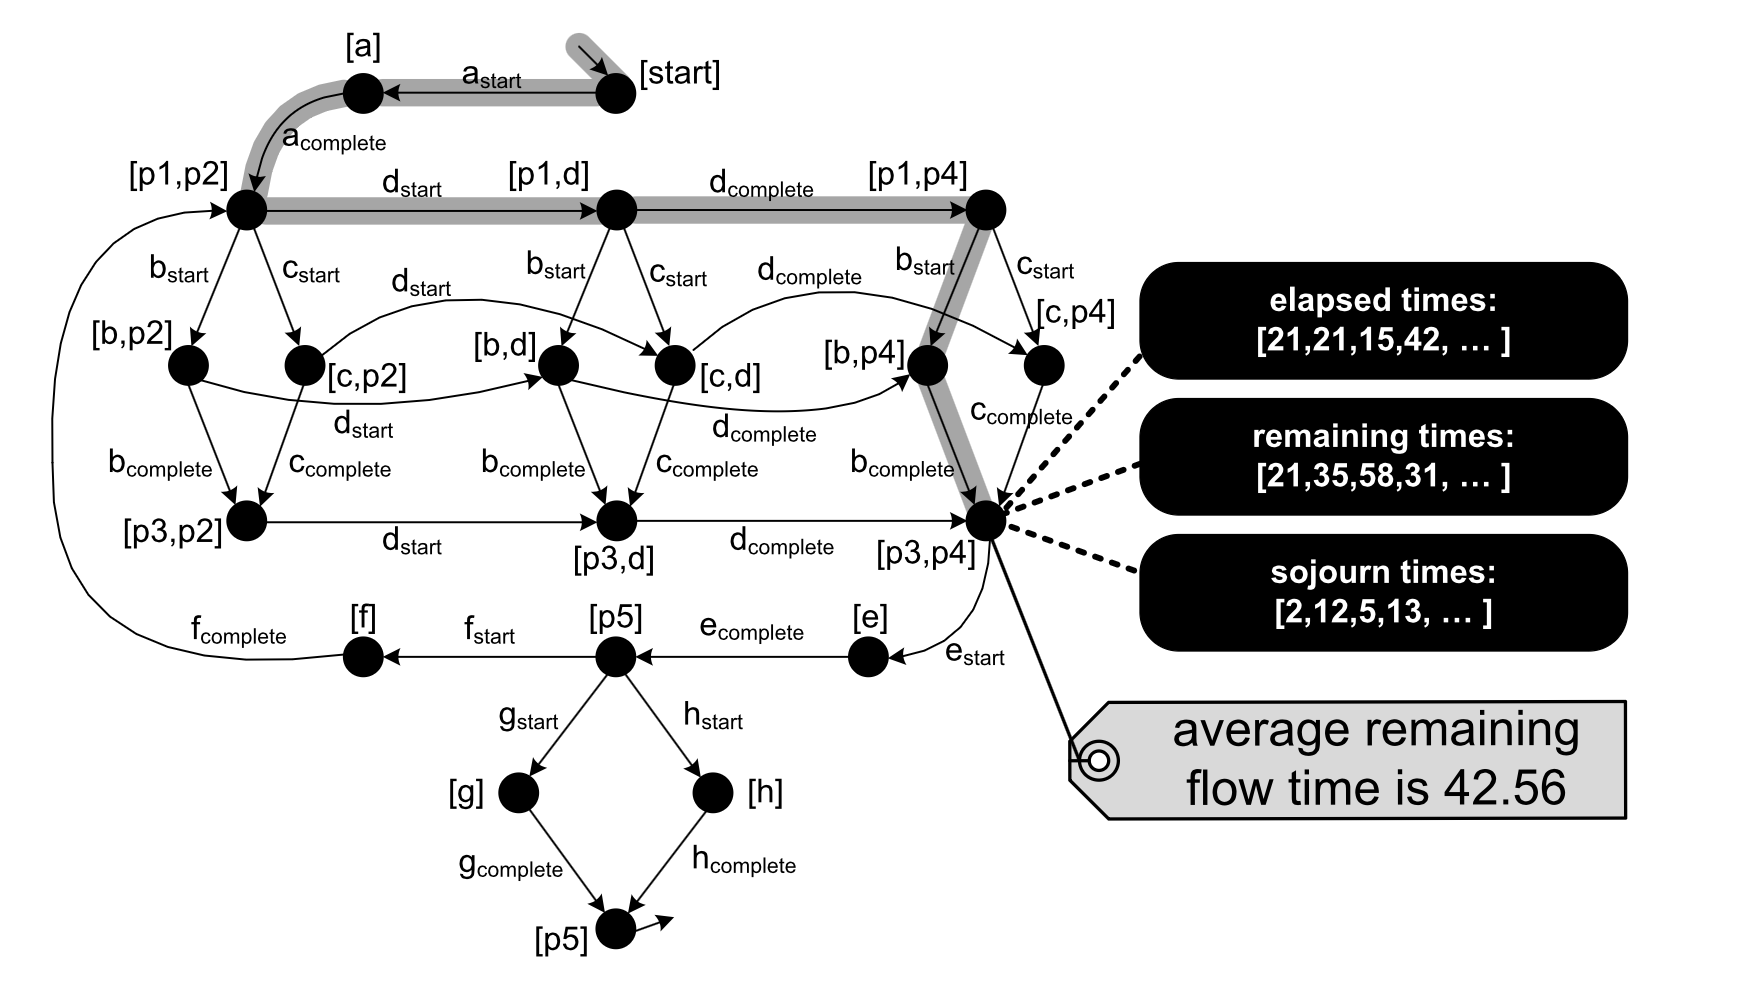
\includegraphics[width=\textwidth]{figures/vanderaalst_states_prediction.png}
	\caption[Transition system with states for remaining time prediction]{
		Transition system annotated with time measurements, taken from \textcite{vanderaalst2016process}. Each node is a state of a running case and each arc is the start or completion of an activity. Each state collects the elapsed, remaining, and sojourn times of all past cases that visited it, as shown for state [p3,p4]. The gray path is a running case that reaches [p3,p4]. Its predicted remaining flow time is 42.56, the average remaining time observed in this state.}
	\label{fig:related_work_states_prediction}
\end{figure}

\section{Event Logs with Known Drifts}
\label{sec:related_work:logs}
\Textcite{adams2023experimental} compare eight detectors only on synthetic event logs with 132 control-flow drifts. None of the detectors performs well on all six evaluation goals, such as accuracy, latency, and robustness to noise. This kind of synthetic logs can be generated by CDLG~\autocite{grimm2022cdlg}: It plays out process trees and injects drifts in the control-flow in four modes. The benchmark by \textcite{padella2026everything}, by contrast, has five real event logs, but with drifts only in control-flow and activity durations. None of these event logs has drifts in the resource perspective or arrival rates. Rheon follows the model of CDLG but adds multiple drift types from all three perspectives supporting sudden and gradual drifts (Chapter~\ref{chap:rheon}).


\section{Positioning of This Thesis}
\label{sec:related_work:positioning}
Three gaps motivate the approach of this thesis:
\begin{itemize}
	\item \emph{Perspectives:} Most detectors detect only control-flow drifts. Detectors for further perspectives recognize drift points in individual features or entire trace distributions but do not describe the process situation compactly.
	\item \emph{States:} Clustering-based detectors mainly cluster control-flow behavior. The state-based works in Section~\ref{sec:related_work:states} use states for prediction, object analysis, or steady-state detection, but not for concept drift detection.
	\item \emph{Test data:} None of the aforementioned works and tools comprise resource drifts or arrival rate drifts.
\end{itemize}
This thesis addresses all three gaps. Our states describe a process in all three perspectives separately (\ref{item:intro:rq_states}), and we evaluate if their changes signal drifts (\ref{item:intro:rq_detection}). Rheon delivers test data with injected drifts in all three perspectives (\ref{item:intro:rg_rheon}).
